

\tikzset{every picture/.style={line width=0.75pt}} %set default line width to 0.75pt        

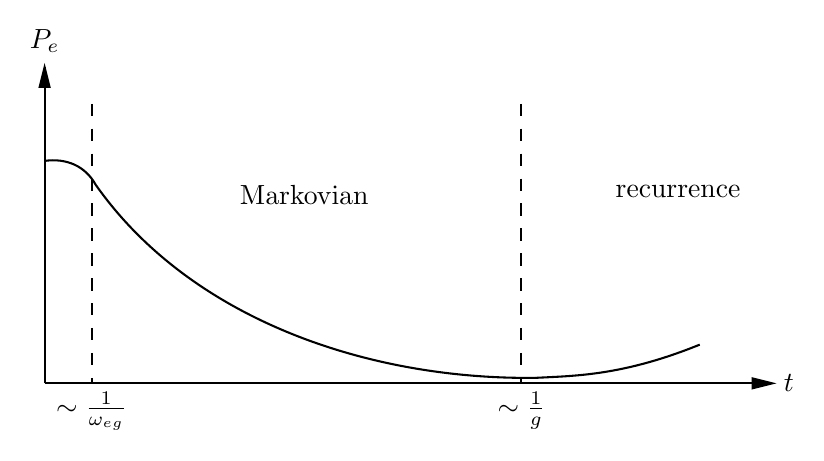
\begin{tikzpicture}[x=0.75pt,y=0.75pt,yscale=-1,xscale=1]
%uncomment if require: \path (0,300); %set diagram left start at 0, and has height of 300

%Straight Lines [id:da3136645111128993] 
\draw    (175.35,229.69) -- (526,229.69) ;
\draw [shift={(528,229.69)}, rotate = 180] [fill={rgb, 255:red, 0; green, 0; blue, 0 }  ][line width=0.08]  [draw opacity=0] (12,-3) -- (0,0) -- (12,3) -- cycle    ;
%Straight Lines [id:da9561030204147447] 
\draw    (175.35,229.69) -- (175.35,77.34) ;
\draw [shift={(175.35,75.34)}, rotate = 90] [fill={rgb, 255:red, 0; green, 0; blue, 0 }  ][line width=0.08]  [draw opacity=0] (12,-3) -- (0,0) -- (12,3) -- cycle    ;
%Curve Lines [id:da24141871701343098] 
\draw    (175.35,122.52) .. controls (186,121.04) and (195,125.04) .. (200,134.04) ;
%Curve Lines [id:da6858896034833271] 
\draw    (200,134.04) .. controls (212.94,152.44) and (229.19,168.04) .. (247.72,180.89) .. controls (293.64,212.73) and (353.58,227.75) .. (412,227.04) ;
%Straight Lines [id:da841804291945832] 
\draw  [dash pattern={on 4.5pt off 4.5pt}]  (198,95) -- (198,229.04) ;
%Straight Lines [id:da39165318886202516] 
\draw  [dash pattern={on 4.5pt off 4.5pt}]  (405,95) -- (405,229.04) ;
%Curve Lines [id:da8947188003962334] 
\draw    (412,227.04) .. controls (431,226.04) and (454,226.04) .. (491,211.04) ;

% Text Node
\draw (175.35,71.94) node [anchor=south] [inner sep=0.75pt]    {$P_{e}$};
% Text Node
\draw (530,229.69) node [anchor=west] [inner sep=0.75pt]    {$t$};
% Text Node
\draw (198,232.44) node [anchor=north] [inner sep=0.75pt]    {$\sim \frac{1}{\omega _{eg}}$};
% Text Node
\draw (405,232.44) node [anchor=north] [inner sep=0.75pt]    {$\sim \frac{1}{g}$};
% Text Node
\draw (268,133) node [anchor=north west][inner sep=0.75pt]   [align=left] {Markovian};
% Text Node
\draw (449,133) node [anchor=north west][inner sep=0.75pt]   [align=left] {recurrence};


\end{tikzpicture}
